\chapter{Analisi dei Risultati}

\section{Metodologia}

In questo capitolo vengono presentati i risultati dell'analisi e le relative interpretazioni. È possibile includere riferimenti al capitolo precedente come Figura~\ref{fig:esempio-figura}.

\begin{figure}[htbp]
    \centering
    
\includegraphics[width=0.7\textwidth]{immagini/placeholder-figure.png}
    \caption{Risultati dell'esperimento principale.}
    \label{fig:risultati-esperimento}
\end{figure}

\subsection{Analisi Statistica}

L'analisi statistica dei dati ha rivelato diverse tendenze significative. Di seguito è riportata una tabella riassuntiva:

\begin{table}[htbp]
    \centering
    \caption{Risultati statistici principali.}
    \label{tab:statistiche}
    \begin{tabular}{lcccc}
        \toprule
        \textbf{Parametro} & \textbf{Min} & \textbf{Max} & \textbf{Media} & \textbf{Dev. Std} \\
        \midrule
        Parametro A & 10.5 & 45.2 & 27.8 & 8.3 \\
        Parametro B & 0.12 & 0.89 & 0.54 & 0.22 \\
        Parametro C & 42 & 128 & 86 & 24 \\
        \bottomrule
    \end{tabular}
\end{table}

\section{Interpretazione dei Dati}

L'interpretazione dei dati raccolti suggerisce che il modello proposto è in grado di generalizzare efficacemente su dataset eterogenei. In particolare, si osserva che:

\begin{itemize}
    \item Il parametro A mostra una correlazione positiva con l'accuratezza del modello
    \item Il parametro B presenta un comportamento non lineare e richiede ulteriori indagini
    \item Il parametro C è risultato meno influente del previsto nelle condizioni sperimentali
\end{itemize}

\subsection{Confronto con lo Stato dell'Arte}

\begin{figure}[htbp]
    \centering
    \begin{subfigure}{0.45\textwidth}
        \centering
        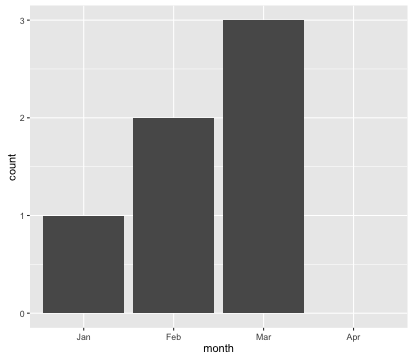
\includegraphics[width=\textwidth]{immagini/placeholder-graph-1.png}
        \caption{Confronto di accuratezza.}
        \label{fig:confronto-accuratezza}
    \end{subfigure}
    \hfill
    \begin{subfigure}{0.45\textwidth}
        \centering
        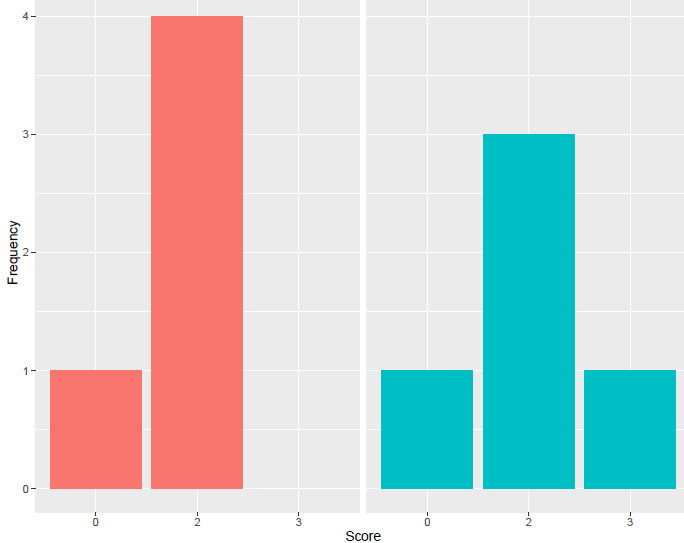
\includegraphics[width=\textwidth]{immagini/placeholder-graph-2.png}
        \caption{Confronto di efficienza.}
        \label{fig:confronto-efficienza}
    \end{subfigure}
    \caption{Confronto con algoritmi esistenti.}
    \label{fig:confronto-completo}
\end{figure}

\section{Limitazioni e Lavori Futuri}

Nonostante i risultati promettenti, il lavoro presenta alcune limitazioni che potrebbero essere affrontate in studi futuri:

\begin{enumerate}
    \item Ampliamento del dataset con casi più eterogenei
    \item Ottimizzazione dell'algoritmo per ridurre il costo computazionale
    \item Estensione del modello per gestire problemi di maggiore complessità
    \item Integrazione con tecniche di apprendimento profondo
\end{enumerate}

\epigraph{La ricerca non è mai finita, ma solo temporaneamente interrotta.}{--- Ricercatore Anonimo}

\section{Conclusioni del Capitolo}

In conclusione, l'analisi condotta in questo capitolo ha evidenziato sia i punti di forza che le limitazioni dell'approccio proposto. I risultati ottenuti suggeriscono che il metodo è promettente ma richiede ulteriori sviluppi per raggiungere il pieno potenziale.

Le direzioni future indicate nella Sezione \ref{fig:confronto-completo} rappresentano il naturale proseguimento di questo lavoro e potrebbero condurre a significativi miglioramenti delle prestazioni.